\section{Approach}
\label{sec:approach}
In this section, we first present a meta-learning framework called model-agnostic meta-learning~\citep{finn2017model}, and then propose the small data text style transfer~(ST$^2$) framework, which adapts meta-learning scheme to effectively exploit relevant knowledge from other style pairs. We then introduce a newly constructed literature translation dataset covering a board range of fine-grained personal writing styles, which can be used to facilitate research in style transfer towards building more practical systems and applications.
\subsection{Preliminary}
%Compared with methods that require multiple layers of operations 
%such as the \emph{Delete-and-Retrieve}~\cite{li2018delete}, 
%much state-of-the-art work use specific model designs to disentangle the style 
%and content in latent space, and used a single-layer model structure. 
%We briefly present two successful single-layer models below.
%Therefore, they are a simple and effective starting point to explore meta-learning framework for the style transfer task. We adapt the \emph{Model Agnostic Meta-learning} scheme on the \emph{CrossAlign} model and \emph{VAE} model in our study~\cite{shen2017style, john2018disentangled}.
%
%\subsubsection*{Cross Align}
%
%The \emph{CrossAlign} model architecture proposed by \citet{shen2017style} is shown in \figref{fig:crossalign}. Let $X$ and $Y$ be two corpus with styles $s_x$ and $s_y$, respectively. $E$ is the encoder that takes source sentence $x$/$y$ and style label $s_x$/$s_y$ as input. The encoded entangled embedding $z_x$/$z_y$ is then combined with its source style label $s_x$/$s_y$ as input to the decoder $D$ to reconstruct the input sentence. Two adversarial discriminators $D_1$ and $D_2$ are introduced to distinguish the hidden state sequence of $D(z_x, s_x)$/$D(z_y, s_y)$ between the hidden state sequence of $D(z_y, s_x)$/$D(z_x, s_y)$, respectively.
%
%\begin{figure}[htbp]
%	\centering
%	\scalebox{1.2}{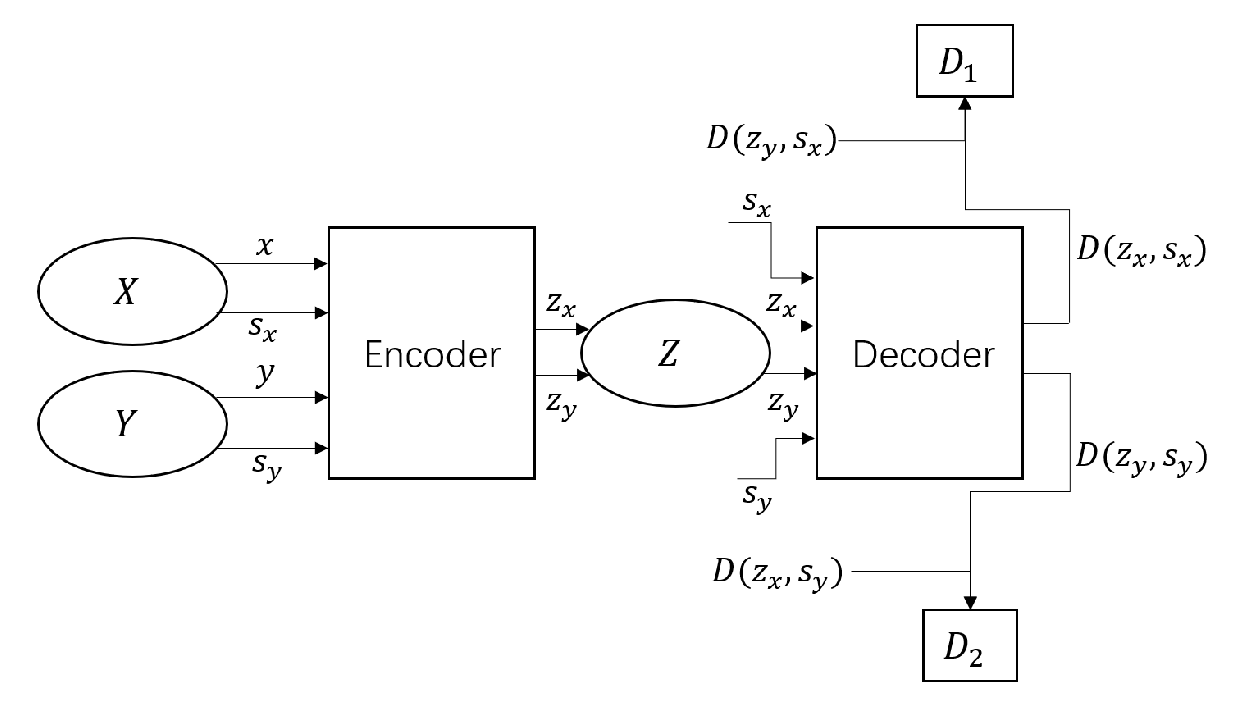
\includegraphics[width=7cm]{./images/cross_align_new_new.eps}}
%	\caption{CrossAlign architecture}
%	\label{fig:crossalign}
%\end{figure}
%
%In training phase, the discriminators and the encoder-decoder model are optimized in an alternate fasion. The objective is to find
%\begin{align*}
%\theta^* = \underset{\theta}{\arg\min\ } \mathcal{L}_{\mathrm{rec}} (\theta_E, \theta_D) &- \mathcal{L} _{\mathrm{adv}}(\theta_E, \theta_{D},\theta_{D_1}) \\
%	&- \mathcal{L}_{\mathrm{adv}}(\theta_E, \theta_D,\theta_{D_2}),
%\end{align*}
%where
%\begin{align*}
%\mathcal{L}_{\mathrm{adv}}(\theta_E, \theta_D,\theta_{D_1}) & = \mathbb{E}_{x\sim X}[-\log D_1(D(E(x, s_x),s_x))] & \\
% + &\mathbb{E}_{y\sim Y}[-\log (1 - D_1(D(E(y, s_y), s_x)))],\\
% \mathcal{L}_{\mathrm{adv}}(\theta_E, \theta_D,\theta_{D_2}) & = \mathbb{E}_{y\sim Y}[-\log D_2(D(E(y, s_y),s_y))] & \\
% + &\mathbb{E}_{x\sim X}[-\log (1 - D_2(D(E(x, s_x), s_y)))]
%\end{align*}
%The discriminators $D_1$ and $D_2$ are both implemented as CNN classifiers~\citep{kim2014convolutional}.
%
%
%\subsubsection*{VAE for Style Transfer}
%
%In order to disentangle style and content in the latent space, \citet{john2018disentangled} used variational autoencoder (VAE) and their specially designed style-oriented and content-oriented losses to guide the updates of the latent space distributions for the two components~\citep{kingma2013auto}. 
%
%The architecture of this model is shown in \figref{fig:vae}. Given a corpus $X$ with unknown latent style space and content space, 
%an RNN encoder maps a sequence $x$ into the latent space, 
%which defines a distribution of style and content~\citep{cho2014learning}. 
%Then style embedding and content embedding are sampled from 
%their corresponding latent distributions and are concatenated 
%as the training sentence embedding. 
%
%The two embeddings are used to calculate multi-task 
%loss $J_{\mathrm{mul}}$ and adversarial loss $J_{\mathrm{adv}}$ 
%for content and style to separate their information. 
%Then this concatenated latent vector is used as a generative 
%latent vector, and is concatenated to every step of the input sequence
%and fed into decoder $D$, which reconstructs the sentence $x'$. 
%The final loss is the sum of these multi-task losses and the usual VAE reconstruction $J_{\mathrm{rec}}$ with 
%KL divergence regularization for both style embedding and content 
%embedding~\citep{kingma2013auto}.
%
%\begin{figure}[htbp]
%	\centering
%	\includegraphics[width=7cm]{./images/vae.pdf}
%	\caption{VAE architecture}
%	\label{fig:vae}
%\end{figure}
%
%
%%The main designs of style- and content-oriented losses are as 
%%follows~\cite{john2018disentangled}.
%%\begin{enumerate}
%%	\item The style embedding should contain enough information to be discriminative. Therefore, a multitask discriminator is added to align the predicted distribution and the ground-truth distribution of labels.
%%	\begin{align*}
%%	J_{\mathrm{mul}}(\theta_E; \theta_{\mathrm{mul(s)}}) = -\sum_{l\in \mathrm{labels}}t_s(l)\log y_s(l),
%%	\end{align*}
%%	where $t_s(l)$ is the distribution of ground-truth style labels, and $y_s(l)$ is the predicted output by the style discriminator.
%%	\item The content embedding should not contain too much style information. Therefore, an adversarial discriminator is added, with loss of the discriminator and adversarial loss for the autoencoder given by
%%	\begin{align*}
%%	J_{\mathrm{dis}(s)}(\theta_{\mathrm{dis}(s)}) & = - \sum_{l\in \mathrm{labels}} t_s(l)\log y_s(l), \\
%%	J_{\mathrm{adv(s)}}(\theta_E) & = -\sum_{l\in \mathrm{labels}}y_s(l)\log y_s(l),
%%	\end{align*}
%%	where $\theta_{\mathrm{dis}(s)}$ contains the weights for a fully connected layer, and $t_c(l)$ is the predicted distribution of style labels when taking content embedding as an input. 
%%	\item The content embedding needs to be able to predict the information given by bag-of-words (BoW), which is defined as
%%	\begin{align*}
%%	t_c(w) := \frac{\sum_{i=1}^N \mathbb{I}\{w_i = w \}}{N},
%%	\end{align*}
%%	for each word $w$ in the vocabulary $V$ with sentence length $N$~\cite{wallach2006topic}. Therefore, a multitask discriminator is added to align the predicted BoW distribution with ground-truth.
%%	\begin{align*}
%%	J_{\mathrm{mul}(c)}(\theta_E; \theta_{\mathrm{mul}(c)}) & = -\sum_{w\in V}t_c(w)\log y_c(w),
%%	\end{align*}
%%	where $t_c(w)$ is the distribution of true BoW representations, and $y_c(w)$ is the predicted output by the content discriminator.
%%	\item The style embedding should not contain content information. Similar as before, an adversarial discriminator is trained to predict the BoW features from style embedding, with loss for discriminator and adversarial loss given by
%%	\begin{align*}
%%	J_{\mathrm{dis}(c)}(\theta_{\mathrm{dis}(c)}) = -\sum_{w\in V}t_c(w)\log y_c(w), \\
%%	J_{\mathrm{adv}(c)}(\theta_E) = -\sum_{w\in V}y_c(l)\log y_c(l).
%%	\end{align*}
%%\end{enumerate}
%
%
%In the training phase, the adversarial discriminators are trained 
%together with other parts of the model, and the final loss of 
%the autoencoder is given by the weighted sum of the loss from traditional VAE, 
%the multitask losses for style and content, 
%and the adversarial losses given by the style and content discriminators. 
%In the inference phase, the style embedding is extracted from the 
%latent space of a target domain and then combined with the original content embedding as input to the decoder.

\subsection*{Model-Agnostic Meta-learning (MAML)}

Meta-learning is the learning paradigm aimed to help a model quickly adapt to a new task, given that it has been trained on several other similar tasks. Compared with other model-based meta-learning methods, model-agnostic meta-learning algorithm (MAML) utilizes only gradient information~\citep{finn2017model}. Therefore, it can be easily applied to models based on gradient descent training.

Given a distribution $p(\mathcal{T})$ over a set of similar tasks, a task-specific loss function $\mathcal{L}_{\mathcal{T}_i}$ and shared initial model parameters $\theta$, we aim to jointly learn a model so that in fine-tuning with the new task, the parameters are well-initialized so that the model quickly converges with fewer epochs and a smaller dataset.

Figure \ref{fig:maml} shows the architecture of MAML. We define the shared model with parameters $\theta$ as a meta-learner. The data for each task is divided into a support set $D_s$ and a query set $D_q$. In each sub-task training, the sub-learner is initialized with the parameters of the meta-learner. Then this parameter is updated $K$ times using the support data for this specific task. After updating, the new parameter is $\theta'_i$ for the $i$-th task, and a loss $\mathcal{L}_{\mathcal{T}_i}(f_{\theta'})$ is evaluated using the query dataset for this sub-task. This sub-training process is performed for each sub-task, and losses from all sub-tasks are aggregated to obtain a loss for meta-training.

\begin{figure}[th]
	\centering
	\includegraphics[width=7cm]{./images/maml.pdf}
	\caption{MAML architecture. For every update of meta-learner's parameters $\theta$, we first update each sub-task on the support dataset $D_s$ for $K$ steps and obtain the new parameter $\theta'$. Then we use the loss evaluated using this new parameter on the query set $D_q$, and sum up all losses from $N$ tasks to update the meta-learner's parameters.}
	\label{fig:maml}
\end{figure}

\begin{algorithm}\small
	\caption{ST$^2$}
	\label{alg:maml}
	\KwIn{a set of style pairs, $\{(s_{t,1}, s_{t,2}), \ldots \}$, where $t = 1, \ldots, N$, parameters $\alpha, \beta$}
	\KwOut{transfer function $f_{\theta}: (x, s) \mapsto y$, where $s$ is the source style, $x$ is the original sentence, $y$ is the transferred sentence in target style}
	\While{not done}{
		\ForEach{style pair $(s_{t,1}, s_{t,2})$}{
			Initialize sub learner with $\theta_t = \theta$\;
			\For{step in 1, \ldots, K}{
				Sample batch data from support set of $t$\;
				Update transfer function $f_{\theta}$ using\\$\qquad\theta_t = \theta_t - \alpha \nabla_{\theta_t}\mathcal{L}_{t}(f_{\theta_t})$\;
			}
			Sample batch data from query set of $t$\;
			Evaluate $\mathcal{L}_t(f_{\theta_t})$\;
		}
		Update meta-learner with $\theta = \theta - \beta\nabla_{\theta}\sum_{t=1}^T \mathcal{L}_t(f_{\theta_t})$\;
	}
\end{algorithm}

\subsection{Small Data Text Style Transfer}
\label{sec:st2}
In contrast to traditional single style pair transfer, in our application, the sub-tasks contain different pairs of styles to be transferred. The meta-learner contains the transfer function 
$f_{\theta}: (x, s)\mapsto x'$, which takes a sentence $x$ with its 
style label $s$, and outputs a sentence $x'$ in the target style with 
similar content. This transfer function is shared by all pairs of styles 
in the meta-training phase. In practice, the transfer function $f_\theta$ can be parameterized by any existing single style pair neural transfer model. In addition, for base models which include adversarial functions for style disentanglement, the updates for the adversarial parameters are also included in the updates of meta-learner. Since the data size for each task with a 
single pair of styles is assumed to be small, 
the goal of ST$^2$ is to transfer knowledge from other style pairs for a better initialization in the fine-tuning phase of a specific sub-task. 
The multi-task style transfer via meta-learning (ST$^2$) algorithm is 
described in Algorithm \ref{alg:maml}. 

\subsection{Literature Translation~(LT) Dataset Construction}
\label{sec:lt}
Current researches on text style transfer generally require large-scale datasets for training, thus they are not able to be applied to personal writing styles. One reason is that personal writing styles are relatively difficult to learn compared to more discriminative styles such as sentiment and formality. Furthermore, sources of data reflecting personal writing styles are quite limited. 

For the reasons above, we attempt to leverage literature translations by different translators as a new challenging text style transfer task. Firstly, there are multiple versions of translation from the same source. Since it is possible to align these comparable sentences to construct ground-truth references, they are well-suited for our test data. Moreover, in addition to the common-source translated work, a translator has other written works, which can be used to serve as a non-parallel training corpus as in standard style transfer setting.
\begin{table*}[!th]
	\renewcommand\tabcolsep{3.0pt} % 调整表格列间的长度
	\scriptsize
	\centering
	\begin{tabular}{c|cccccccccccc}
		\hline
		\multirow{2}{*}{\textbf{Statistics}}  & \multirow{2}{*}{\shortstack{Alban\\Kraisheime}}  & \multirow{2}{*}{\shortstack{Isabel\\F.Hapgood}} & \multirow{2}{*}{\shortstack{Andrew\\R. MacAndrew}} &\multirow{2}{*}{\shortstack{Richard\\Pevear}} &\multirow{2}{*}{\shortstack{David\\Hawkes}} &\multirow{2}{*}{\shortstack{Yang\\Xianyi}}
		&\multirow{2}{*}{\shortstack{John\\E. Woods}} &\multirow{2}{*}{\shortstack{H. T.\\Lowe-Porter}} &\multirow{2}{*}{\shortstack{Ian C.\\Johnston}} & \multirow{2}{*}{\shortstack{Robert\\Fagles}} &\multirow{2}{*}{\shortstack{Julie\\Rose}}
		&\multirow{2}{*}{\shortstack{Michael\\R. Katz}}\\
		& & & & & & & & & & & &\\
		\hline
		Vocab Size & 16,810 & 17,205 & 11,814 & 14,831 &15,121 &11,436 &21,869 &20,819 &11,168 &13,521 &18,020 &13,908\\
		Average Length &20.9   &20.4  &19.5 &20.7 &18.6 &15.9 &25.1 &26.7 &13.5 &26.6 &20.0 &19.0\\
		\# of Adjectives &11,798   &11,187   &10,050 &11,364 &9,622 &7,581 &17,521 &19,187 &8,236 &15,246 &11,255 &11,283\\
		\# of Adverbs &9,462   &8,325  &14,848  &13,580 &10,622 &9,555 &14,667 &17,369 &7,901 &13,991 &9,362 &13,506\\
		\# of Conjunctions &22,649  &20,673 &16,640  &19,675 &17,086 &13,762 &25,837 &26,789 &13,916 &27,801 &20,112 &16,650\\
		Flesch Readability &68.7 &66.7 &71.1 &67.4 &73.0 &79.6 &61.3 &59.6 &79.8 &70.2 &70.6 &66.4\\
		Dale-Chall Readability &6.2 &6.3 &5.2 &5.7 &5.4 &4.9 &6.5 &6.7 &5.2 &6.1 &5.8 &5.9 \\
		\hline
	\end{tabular}
	\caption{Linguistic statistics of each writer. The higher the Flesch readability, the easier it is to read. The Dale-Chall readability score indicates the grade level required to understand the text. See \url{https://en.wikipedia.org/wiki/Dale-Chall_readability_formula} for full description.}\label{tb:stats}
\end{table*}
\begin{table*}[!th]
	\centering
	\small
	\begin{tabular}{c|c}
		\hline
		\multicolumn{2}{c}{\textbf{The Iliad}~(Ian C. Johnston$\leftarrow$$\rightarrow$Robert Fagles)}\\
		\hline
		\emph{there are none left for us to pass around .} & \emph{no time for rest .} \\
		\emph{so sit down quietly.do as i say .} & \emph{now go sit down .} \\
		\emph{troops assembled on the run .} & \emph{ the troops assembled .} \\
		\emph{but soon enough he 'd rouse himself again .} & \emph{perhaps he will be persuaded .} \\
		\emph{as far as i 'm concerned , it ’ s not your fault .} & \emph{you are not to blame .} \\
		\emph{but things did n't work that way .} & \emph{we can not find a thing .} \\
		\emph{you 've come back from the fight .} & \emph{we 'll fight again tomorrow .} \\
		\emph{don't upset .} & \emph{no , do n't give up now .} \\
		\hline
	\end{tabular}
	\caption{Samples drawn from the common source The Iliad out of Literature Translation(LT) dataset. Left panel shows the translation by Ian C. Johnston and right panel shows the translation by Robert Fagles.}
	\label{table:LT}
\end{table*}
We align sentences for each style pair using the algorithm provided by \citet{chen2019align} for testing. The sentence pairs are extracted from the common translated work for each writer pair. The test data has approximately 1k sentences for each writer. Table \ref{table:LT} gives some sample aligned sentences in the test set. While it is generally difficult to characterize different writing styles using discrete representation, we also report some statistics regarding each writer's translation. For example, Ian C. Johnston tends to use more concise expressions(13.4 v.s. 26.6 tokens per sentence) than Robert Fagles even they possess similar vocabulary(11168 v.s. 13521) when translating \textit{The Iliad}. More detailed statistics can be found in Table \ref{tb:stats}.
\begin{table}[t]\scriptsize
	\centering
	\begin{tabular}{c|cc}
		\hline
		\textbf{Common Source} & \textbf{Writer A} & \textbf{Writer B} \\
		\hline
		Notre-Dame de Paris & Alban Kraisheimer & Isabel F. Hapgood \\
		The Brothers Karamazov & Andrew R. MacAndrew & Richard Pevear \\
		The Story of Stone & David Hawkes & Yang Xianyi \\
		The Magic Mountain & John E. Woods & H. T. Lowe-Porter \\
		The Iliad & Ian C. Johnston & Robert Fagles \\
		Les Miserables & Isabel F. Hapgood & Julie Rose \\
		Crime and Punishment & Michael R. Katz & Richard Pevear \\
		\hline
	\end{tabular}
	\caption{Literature Translations(LT) dataset. The first column shows the name of translated works with common source for the two writers in the same row.}\label{tb:translations}
\end{table}
We collect a set of writers with unknown different writing styles $\{s_1, \ldots, s_n\}$, with each writer has his/her own set of written works $\{c_{s_i, 1}, \ldots, c_{s_i, n_i} \}$. In order to have a test set with ground-truth references, we used translated works from non-English sources\footnote{Obtained from \texttt{http://gen.lib.rus.ec/}.}, so that each writer in our set has at least one translated work that is from the same source as another writer~(see Table \ref{tb:translations}). Namely, for each writing style $s_i$ in the set, there exists another style $s_j$ and $\exists\ k_1, k_2$ such that $src(c_{s_i, k_1}) = src(c_{s_j, k_2})$. In this dataset, each writer has approximately 10k non-parallel sentences for training.


%\begin{table}[th]
%	\small
%	\centering
%	\begin{tabular}{c|cc}
%		\hline
%		\textbf{Writer} & \textbf{Vocab Size} & \textbf{Avg.SentLen} \\
%		\hline
%		Alban Kraisheime &16,810  &20.9  \\
%		Isabel F. Hapgood &17,205  &20.4  \\
%		Andrew R. MacAndrew &11,814  &19.5  \\
%		Richard Pevear &14,831  &20.7  \\
%		David Hawkes &15,121  &18.6  \\
%		Yang Xianyi &11,436  &15.9  \\
%		John E. Woods &21,869 &25.1  \\
%		H. T. Lowe-Porter &20,819 &26.7 \\
%		Ian C. Johnston &11,168 &13.5 \\
%		Robert Fagles &13,521 &26.6 \\
%		Isabel F. Hapgood &17,205 &20.5 \\
%		Julie Rose &18,020 &20.0 \\
%		Michael R. Katz &13,908 &19.0 \\
%		\hline
%	\end{tabular}
%	\caption{Statistics regarding the writing style of each writer.}\label{tb:translations}
%\end{table}

